\section{Experiment 9B: robustness of learned compatibility groups}
\label{sec:experiment9b}

\paragraph{Question and frozen gate.}
Experiment 9B tests whether the successful label-free parameter clustering of
Experiment 9A survives four departures from its favorable benchmark: very
short local records, increased measurement noise, strongly unbalanced family
sizes, and a population with continuous rather than discrete heterogeneity.
Privacy and the rejected control-weighted metric remain excluded so that this
experiment isolates the reliability of group discovery. Ten fresh training and
test fleet pairs (seeds 126--135) are used in every regime.

For the discrete regimes, Learned-$K$ must remain within 5\% of Oracle family,
reach unseen-client ARI of at least 0.9, remain feasible and frozen-stable, and
use fewer models than Local. For the continuous regime, where no family labels
exist, the reference partition is selected from the unobserved true parameter
ratios by the same rule. Learned-$K$ must remain within 5\% of that oracle-
information partition and improve on Global by at least 20\%. These gates were
fixed before running the experiment.

\paragraph{Protocol.}
The baseline uses 180 balanced training clients, 30 unseen test clients, three
one-second single-speed records per client, and output-noise standard deviations
of $0.05^\circ$ and $0.1^\circ$. Short-data reduces each record to 0.25~s;
high-noise increases the two noise levels to $0.2^\circ$ and $0.4^\circ$.
Unbalanced populations use 100, 60, and 20 training clients and 15, 10, and 5
test clients in the three latent families. The continuous population
interpolates physical vehicle parameters between handling and heavy endpoints,
adds small independent scatter, and supplies no class labels. The selection
rule remains silhouette maximization over $K=2,\ldots,8$, with minimum
silhouette 0.25 and at least ten training clients per cluster. All final control
tests use the nonlinear tire plant and three held-out maneuvers.

\begin{table}[htbp]
\centering
\caption{Experiment 9B learned-group robustness. Tracking cost is relative to
Oracle family for discrete regimes and the true-ratio partition for the
continuous regime.}
\label{tab:experiment9b-gates}
\begin{tabular}{lrrrrr}
\toprule
Regime & Learned tracking & $K$ range & Reference cost & Global gain & Gate\\
\midrule
Baseline & 0.007583 & 3--3 & $+0.08\%$ & $35.66\%$ & pass\\
Short data & 0.012441 & 2--7 & $+63.87\%$ & $-7.46\%$ & fail\\
High noise & 0.009184 & 2--6 & $+21.90\%$ & $21.82\%$ & fail\\
Unbalanced & 0.007551 & 2--3 & $+1.49\%$ & $21.08\%$ & pass\\
Continuous & 0.007662 & 2--2 & $-0.42\%$ & $17.25\%$ & fail\\
\bottomrule
\end{tabular}
\end{table}

\begin{table}[htbp]
\centering
\caption{Partition diagnostics for the learned estimator. ARI is defined only
for the discrete-family regimes and is used only for their frozen gate.}
\label{tab:experiment9b-clusters}
\begin{tabular}{lrrr}
\toprule
Regime & Mean $K$ & Test ARI & Silhouette\\
\midrule
Baseline & 3.0 & 0.980 & 0.538\\
Short data & 3.2 & 0.082 & 0.349\\
High noise & 2.8 & 0.390 & 0.356\\
Unbalanced & 2.9 & 0.954 & 0.530\\
Continuous & 2.0 & --- & 0.513\\
\bottomrule
\end{tabular}
\end{table}

\begin{figure}[htbp]
\centering
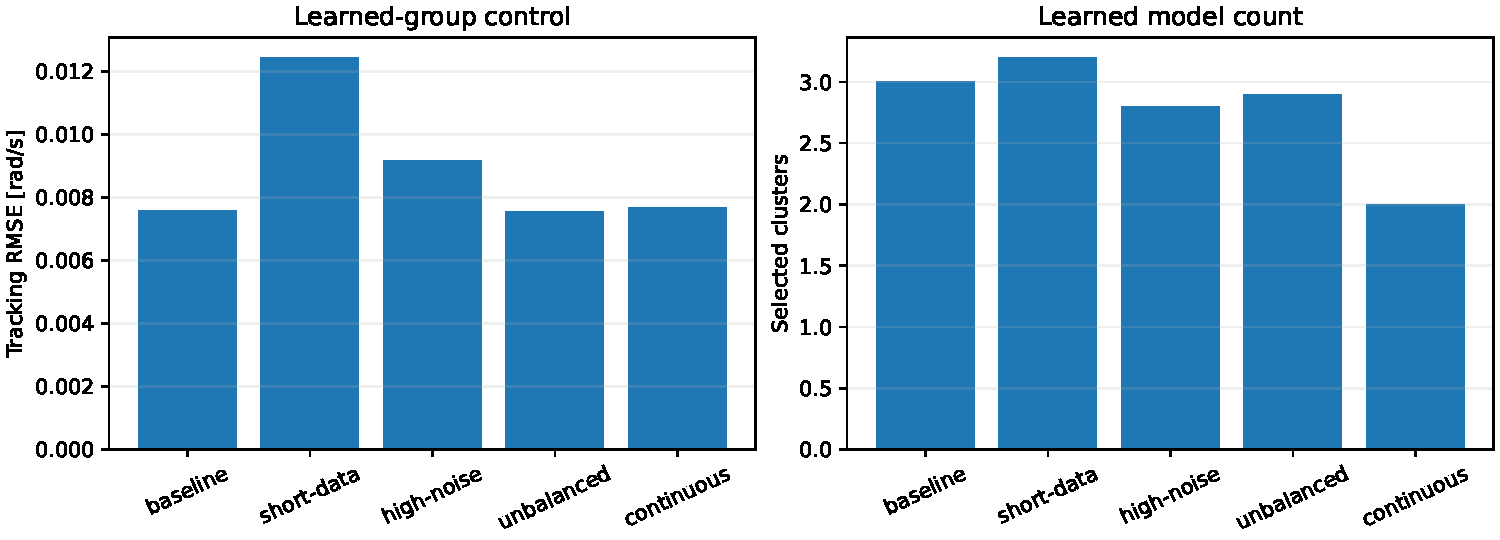
\includegraphics[width=0.93\linewidth]{../results/figures/experiment_9b_group_robustness.pdf}
\caption{Tracking and selected model count under the five Experiment 9B
regimes. The continuous population is represented by two learned regions, not
interpreted as two physical families.}
\label{fig:experiment9b}
\end{figure}

\paragraph{Results.}
All 10,500 local identification fits converge. All 21,600 nonlinear closed-loop
evaluations are amplitude-feasible, and every audited frozen closed-loop radius
is below one. Baseline replicates the 9A result: three groups are always selected,
unseen ARI is 0.980, and tracking is within 0.08\% of Oracle family. The highly
unbalanced case also passes, despite selecting two groups in one fleet; its mean
unseen ARI is 0.954 and its tracking cost is 1.49\%.

Short-data and high-noise fail decisively. With 0.25~s records, selected $K$
ranges from two to seven and unseen ARI falls to 0.082. Learned grouping is
63.87\% worse than Oracle family and 7.46\% worse than Global. It is nevertheless
6.70\% better than the highly uncertain Local models, showing variance reduction
without reliable compatibility discovery. Under high noise, unseen ARI is 0.390
and the tracking cost relative to Oracle family is 21.90\%.

For continuous heterogeneity, both estimated-parameter and true-ratio selection
choose two regions in every fleet. Learned-$K$ is 0.42\% better than the oracle-
information partition and uses two rather than 30 Local controllers. Its
17.25\% improvement over Global, however, misses the frozen 20\% requirement.
This is evidence that coarse region sharing remains useful without natural
families, but not a passed robustness claim. Local tracking remains best in
absolute terms in this regime.

\paragraph{Decision and paper implication.}
The omnibus robustness gate fails: ordinary point-estimate clustering is
credible for adequately informative records, including strong population
imbalance, but is not robust to severe local estimation uncertainty. Thus the
paper must not claim generally reliable automatic family discovery. A defensible
claim is narrower: label-free compatibility discovery can reproduce oracle
sharing in informative regimes and reveals useful coarse regions under
continuous heterogeneity. The next methodological experiment should make the
partition uncertainty-aware---for example by repeated local estimates or
fit-covariance-aware distances---and test recovery on the frozen short-data and
high-noise cases. Private clustering should follow, rather than compound, this
identified weakness.

\paragraph{Reproducibility.}
The frozen protocol is in \path{code/config/experiment_9b.json}; implementation
is in \path{code/experiments/experiment_9b_group_robustness.py}. Aggregate
tables, per-seed summaries, gate decisions, and provenance hashes are retained
under \path{results/tables}.
